\chapter{Single dimension experiments \label{sec:singleDimension}}\thispagestyle{empty}
\par{
    This chapter discusses the results of several experiments in the construction of single-dimensional models.
    The objective of these experiments is to investigate the influence different model hyperparameters have on the model performance.
    Based on this investigation, the hyperparameters for the single-dimensional models in the final step can be chosen.  
}
\section{Single dimension weakly supervised models}
\par{
    In this section, the results of experiments with different model hyperparameters are compared to each other.
    The point annotation sets are generated from the available full annotation masks for each slice.
    In this work, different datasets were used with different levels of provided annotation. 
    Annotation differences between different datasets are listed in table \ref{tab:datasetReferences} on page \pageref{tab:datasetReferences}.
}
\par{
    For three datasets\footnote{The three datasets for which complete annotation is available are the xVertSeg dataset, the UniSiegen dataset and the MyoSegmentum dataset. Of which the MyoSegmentum dataset is the largest by far.},
    full annotation masks are available, meaning that these scan volumes are labelled with volumes for each of the five lumbar vertebrae.
    For each voxel, the ground truth indicates whether it belongs to a lumbar vertebra and which vertebra.
    For one dataset (PLoS), only semantic segmentation is available. It means that the lumbar vertebrae are indicated as one class but not distinguished. 
    With each voxel in the PLoS dataset, ground truth is associated that indicates if it belongs to a lumbar vertebra. There is no label, however, to indicate which of the lumbar vertebrae this is.
}
\par{
    When a scan is sliced along the craniocaudal axis\footnote{
        The nomenclature of anatomical planes and axis is illustrated in figure \ref{fig:anatomicalPlains} on page \pageref{fig:anatomicalPlains}.
        The craniocaudal axis is the vertical axis when the patient is standing up.} 
    a human can distinguish all five lumbar vertebrae (after some practice).
    Therefore, one may hope the single-dimension models trained on sagittal or frontal slices will be able to do the same.
    Even though delineating a vertebra on a transverse slice is possible, identifying which vertebra is presented is challenging for a human.
    Supported by a brief test, it was confirmed that trying to estimate five vertebra classes from the transverse slices only provides very confusing results.
    The models trained on the transverse slices only intend to label the slice pixels as either background (0) or vertebra (1), 
    whereas the models trained on the sagittal and frontal slices intend to indicate which of 6 classes\footnote{0 for background and $i\in [1,2,3,4,5]$ for the corresponding $L i \in [L1,L2, L3, L4, L5]$.} the pixel belongs to.
}
\par{
    The models trained to segment sagittal and frontal slices were trained on datasets xVertSeg, UniSiegen and MyoSegmenTUM.
    From the available full masks, point annotation labels were extracted.
    The models trained to segment transverse slices\footnote{This segmentation is, as stated not based on distinguishing separate lumbar vertebrae from each other.} 
    are trained on the same three datasets and additionally on the PLoS dataset.    
}
\par{
    The model performance results are compared based on the weighted dice score calculated on the test set.
    This metric is described in chapter \ref{sec:dice} on page \pageref{sec:dice}.
}
\subsection{Evaluation of the model Hyperparameters}
\par{
    Several tests were conducted to estimate the influence of model components and model hyperparameters\footnote{
        One could argue that the number of annotation points is not a \textit{model} hyperparameter. It is an essential parameter for the \textit{modelling} approach in general.
    } on the model performance.
}
\subsubsection{Weighted vs unweighted point loss performance}
\par{
    Equation \ref{eq:LP} on page \pageref{eq:LP} defines the point loss $\mathcal{L}_P$. 
    In this equation, the factor $w_{\mathcal{Y}_i(\vec{p})}$ indicates a weight that can be assigned to each of the output classes.
    Since data classes can be unbalanced, these weights can help to counter this imbalance.
    In this problem (based on the available datasets), there are about 500 times more background voxels than voxels belonging to a lumbar vertebra.
    By weighing with a factor proportional\footnote{The weighting vector is normalized.} to this ratio, this imbalance can be countered\footnote{
        When full data labels are available, the counts of the voxel types are available for the train set (one should not include the counts of the validation \& test set to avoid data leakage).
        In principle, this information is not necessarily available when only point level annotation is available. In this work, it is considered that (at least an approximation) of the ratios can be available as prior knowledge.
    }. In the unweighted case, $w_{\cdot} = 1$.
}



\par{
    In figure \ref{fig:weighted_vs_unweighted}, the difference between the weighted dice score \& the average dice score on the test set is compared for two models trained on the transverse slices.
    This result shows that the result of the non-weighted segmentation is better than the result of the model trained with weighted loss.
    At first, this seemed surprising.
    Contrary to fully supervised models, in the weakly supervised case, the ratio between \textit{labelled} points is not as unbalanced as the ratio between the actual class pixels in the result.
    This explains the weighted point loss performance compared to the unweighted point loss performance.
    An approach that is not tested in this work is to weigh proportional to the inverse of the number of \textit{annotation} points per class instead of weighing proportional to the number of \textit{ground truth} pixels\footnote{
        It seems worthwhile for future researchers to investigate such an approach deeper. 
        As it is clear from this chapter and chapter \ref{sec:numberofpoints}, extracting more annotation points (or asking the expert to provide more annotation points) does not necessarily guarantee a better model performance.
    }.
    The disappointing performance of the model trained with a weighted point loss compared to the model trained with the unweighted point loss was  investigated deeper.
    Due to the overweighing of the classes, the model trained with the weighted point loss does not predict the background class anymore! 
    This results in a recall score of 0.00 for this class.
    Based on these observations, the subsequent models in this work are trained with the non-weighted point loss component.
    As mentioned earlier, one could investigate other weighting schemes to optimize concerning the point labels provided.
    Even though this is an interesting topic, it was not investigated further in this work.
}
\begin{SCfigure}[][htb]
    \centering
    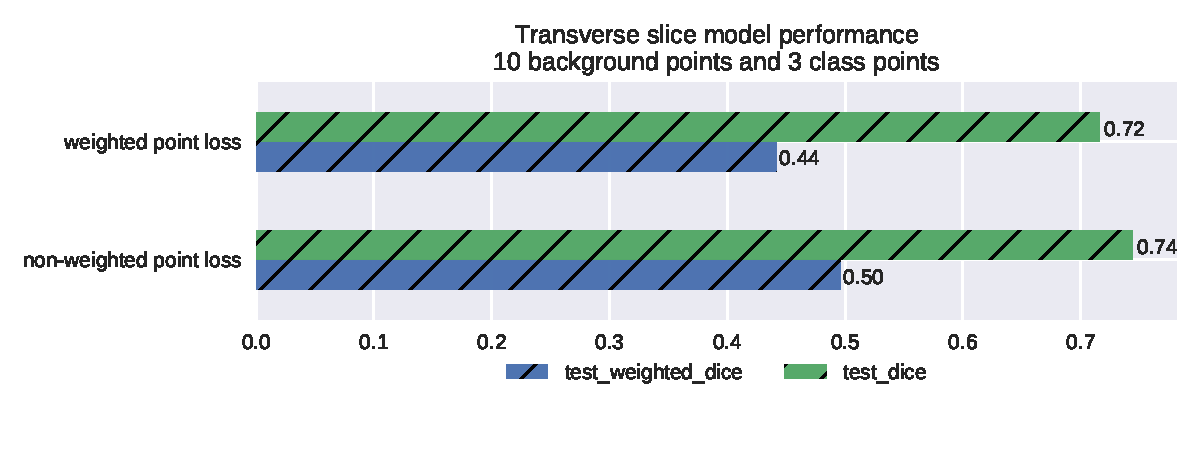
\includegraphics[width=.95\textwidth]{images/weightedvsnonweighted_transverse.pdf}
    \caption{
        Illustration of the difference in model performance (inverse class weighted dice score) between a weighted point loss function and the unweighted point loss function for point annotated models trained on transverse slices.
    \label{fig:weighted_vs_unweighted_transverse}}
\end{SCfigure}%
\begin{SCfigure}[][htb]
    \centering
    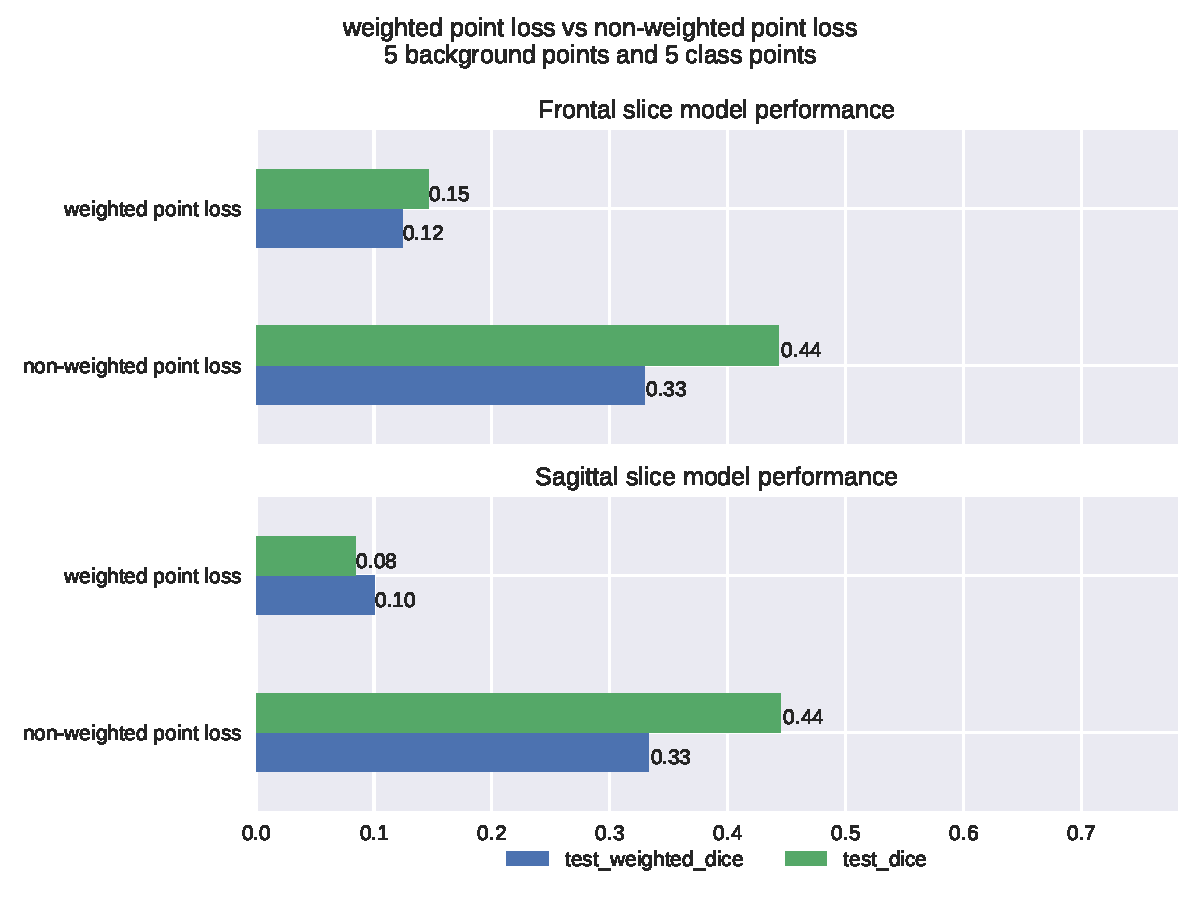
\includegraphics[width=.95\textwidth]{images/weightedvsnonweighted.pdf}
    \caption{
        Illustration of the difference in model performance between a weighted point loss function and the unweighted point loss function for point annotated models trained on frontal slices.
        The models are trained with point annotations extracted from the available ground truth masks. For these models, 
        5 points were extracted from the background mask and 5 points were extracted from each instance of each class in the slice. 
        The bar in blue indicates the inverse weighted dice score, evaluated on the test set. The bar in green indicates the average dice score over the classes.
        \label{fig:weighted_vs_unweighted}}
\end{SCfigure}

Figure \ref{fig:weighted_vs_unweighted_transverse} shows the result of models trained on the same datasets of transverse slices.
These models are trained with point annotations extracted from the available ground truth masks. For these models, 
10 points were extracted from the background mask, and 3 points from each instance of each class in the slice. 
The texture on the plots of the transverse model performance bars tries to help the reader identify that these models do not distinguish the vertebrae from each other but only predict a voxel to be a vertebra or not.
Figure \ref{fig:weighted_vs_unweighted} shows the result for transverse slices.
Remark that the number of class annotation points and background points is different between figure \ref{fig:weighted_vs_unweighted_transverse} and figure \ref{fig:weighted_vs_unweighted}.


\subsubsection{Value of the added loss components}
\par{
    In this work, two-loss components were added to the consistency loss published in \cite{Laradji2021}.
    Where \cite{Laradji2021} is based only on the point loss $\mathcal{L}_P$, and the consistency loss $\mathcal{L}_C$, this work makes use of two extra loss components:
    the prior extend loss $\mathcal{L}_E$ and the separation loss $\mathcal{L}_S$. The four-loss components used in this work are described in more detail in \ref{sec:LossFunctions}.
    Figure \ref{fig:addedLossComponents} shows experimental results validating the positive influence these added loss terms have on the model performance.
}
\begin{SCfigure}[][htb]
    \centering
    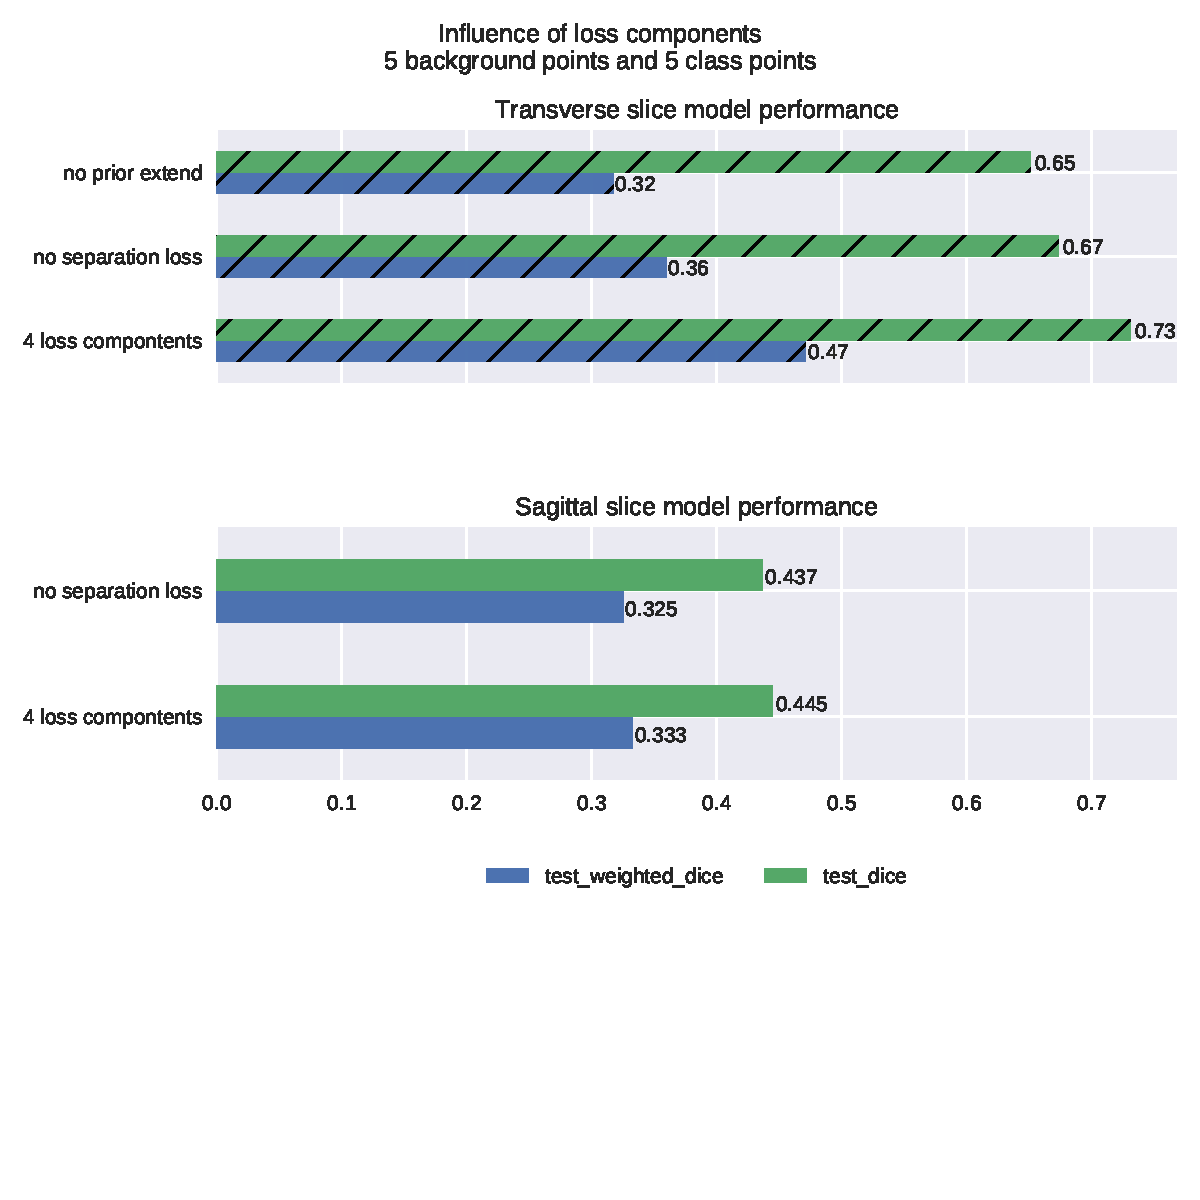
\includegraphics[width=.95\textwidth]{images/Losscomponents.pdf}
    \caption{Evaluation of the added value of loss components. 
    The bar in blue indicates the inverse weighted dice score, evaluated on the test set. The bar in green indicates the average dice score over the classes.
    The texture on the bars representing the transverse model performance help the reader remember the transverse model does not distinguish between the lumbar vertebrae.
    \label{fig:addedLossComponents}}
\end{SCfigure}

\subsection{Evolution of the model performance with increased labelling effort\label{sec:numberofpoints}}
\par{
    The most basic modelling hyperparameter for a point annotation modelling campaign is the number of labelling points one asks the expert to provide.
    This section presents experimental results to estimate the number of annotation points on the resulting model performance.
    Intuitively, one would expect the model performance to increase with the number of annotation points provided.
    This hypothesis turns out to be false.
}
\begin{SCfigure}[][htb]
    \centering
    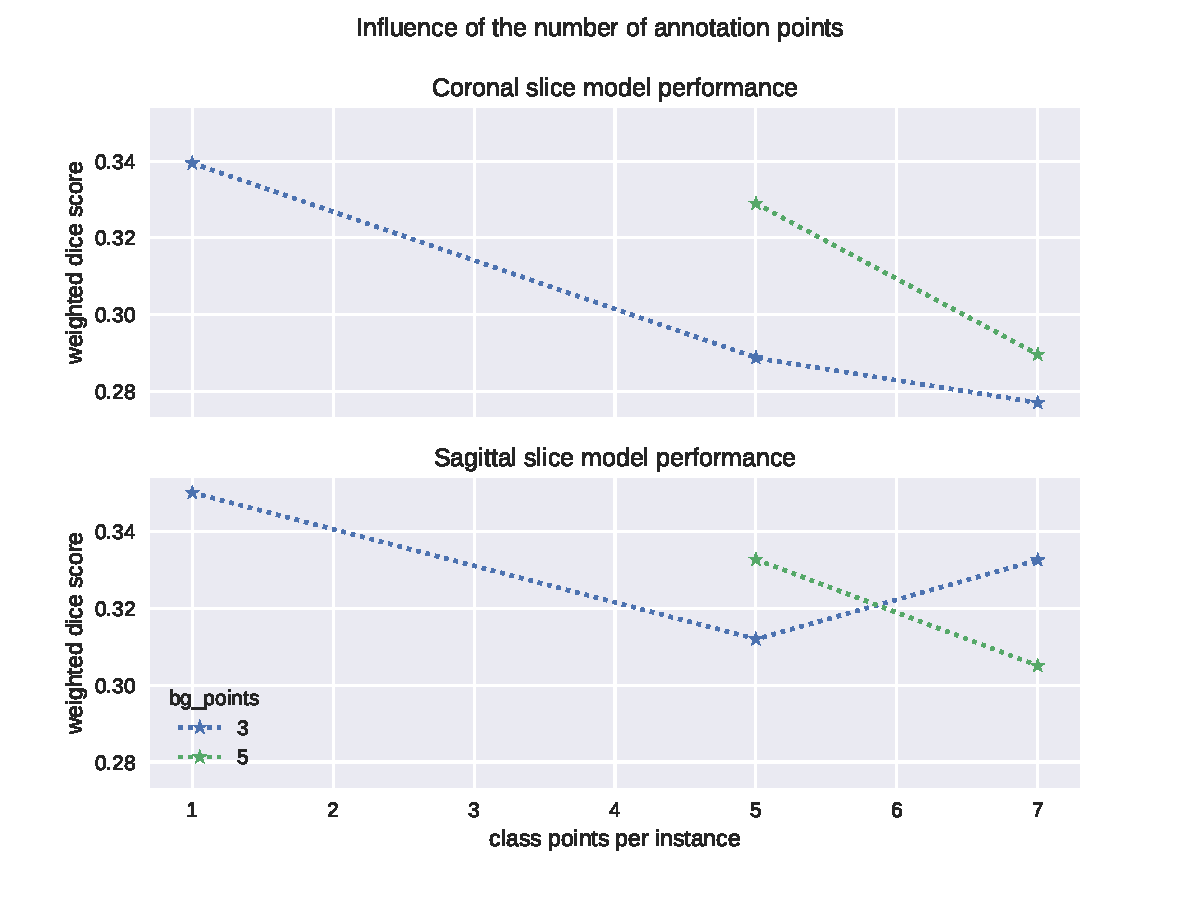
\includegraphics[width=.95\textwidth]{images/BlobPoints_influence.pdf}
    \caption{Evolution of the weakly supervised model performance with increased number of annotation points on the inverse class weighted dice score of the point annotated models.
    Eventhough increasing the number of class annotation points does not improve the model performance, there seems to be an increase in model performance possible by increasing the number of background points.
    \label{fig:points_influence}}
\end{SCfigure}

\par{
    Figure \ref{fig:addedLossComponents} shows the weighted dice score decreases with more annotation points for models trained with unweighted point loss.
    The model becomes very eager to find class points. This causes many background pixels to be wrongly classified as class points.
    The resulting decrease in precision causes the F1 score to decrease.
    It might be interesting for future researchers to investigate the influence of relative quantity of class and background annotation points.
    The time (and computational power) to investigate this behaviour completely was not available in this thesis project.
}